% Chapter 44: The Schrödinger Equation: How Quantum States Evolve
\chapter[The Schrödinger Equation]{The Schrödinger Equation: How Quantum States Evolve}

Chapter~42 showed classical defeats in blackbody radiation, photoelectricity, and atomic spectra. Chapter~43 supplied new bookkeeping: wavefunctions represent states, squared amplitude moduli give probabilities, and complex numbers record phases. But that ledger was static, predicting only present measurements. A complete theory must answer our recurring second question: \emph{what law determines how states change?} Newton answers with \(F=ma\); quantum mechanics uses an energy-driven equation, this chapter's protagonist. By the end you will know why differently sized particles of one material glow in different colors, why microscopic notes never go out of tune, and why your USB drive will eventually forget its contents.

\step{A Counterintuitive Opening}

Start with something perhaps already in your home. Premium LCD televisions advertise quantum dots, billions of semiconductor nanoparticles such as cadmium selenide. Remarkably, grind them to two or three nanometers and they glow blue; five or six, green; larger, red. \emph{Identical chemistry, with particle size the sole variable.} Childhood teaches material determines color: yellow gold, red copper, blue copper sulfate solution. At nanoscales, materials surrender authority to box size. Color is frequency, quantum frequency is energy: an electron's energy is dictated by its home's dimensions. No classical counterpart exists: a marble's energy depends on how hard you throw it, not the size of its box.

Now the reverse, astonishing constancy. Excited hydrogen emits distinctive red light near \(656.3\) nanometers. A laboratory hydrogen lamp gives this wavelength; galaxies over ten billion light-years away give exactly the same decimal digits after redshift correction. Physicists exploit this stability: strontium clocks time an atomic transition with uncertainty below \(10^{-18}\). Running from the Big Bang to now and through that duration again would accumulate under one second of error. Macroscopic strings loosen, springs soften, and crystal oscillators age. Microscopic states can seem frozen by time, never detuning.

One phenomenon lets size dictate energy; the other lets states defy time. Explaining both requires the law of quantum-state evolution.

\step{Make a Guess First}

Place your bets as usual.

First: trap an electron in an inescapable box and halve its width. Does energy (a) stay unchanged, (b) double, (c) quadruple, or (d) decrease?

Second: a slow ball rolling up a hill must return, classically forbidden to cross without enough energy. Can an electron appear beyond a potential wall exceeding its energy? (a) Never; (b) with a small probability; or (c) certainly?

Third: stationary states have time-independent probability distributions. Is their electron (a) fixed at one position, (b) still restless with nonzero kinetic energy, or (c) is everything motionless because probability is?

Fourth: superpose two individually unchanging stationary states in fixed proportions. Is the result (a) necessarily unchanged, since unchanged plus unchanged stays unchanged, or (b) oscillatory? Think carefully: this is a trap for intuition.

Record all four for the final accounting.

\step{Hands-on Experiment}

\begin{experiment}[A Rubber Band's Musical Scale]
\textbf{Materials}: a thick rubber band or any guitar or ukulele string, a table, and a phone, preferably with slow-motion video.

\textbf{Step one}: stretch and fix the band across the table with tape or books, taut enough to sound clearly when plucked. Pluck its center and watch one full arch vibrate up and down.

\textbf{Step two}: \emph{lightly} touch the midpoint, without pressing firmly, and pluck one half. An octave-higher tone sounds. Look closely or film slowly: opposite arches vibrate on either side while the middle stays still. Touch one-third and pluck for another tone and three segments.

\textbf{Step three}: move one anchor inward to halve the vibrating length and pluck the whole: pitch roughly doubles.

\textbf{Step four}: try an arbitrary shape, pressing firmly at \(37\%\) before release. The shape immediately spreads, wobbles, and reorganizes into confused vibration without a clean note.

\textbf{Record and think}: why do only integer-segment shapes persist while arbitrary ones cannot survive an instant? How do length and pitch relate? Remember both observations and mentally replace string length by the electron's box and pitch by its energy. Your rubber band previews our equation macroscopically.
\end{experiment}

\step{The Old Model Runs into Trouble}

Before finding new evolution, explain why old laws fail. Try the candidates.

\textbf{Candidate one: Newton's second law.} Its present consists of position and velocity; force takes over their future. Chapter~43 condemned this picture: electrons have no secret definite trajectories, as double-slit fringes prove. The entire wavefunction map is the state, so the new law takes a map, not two numbers. Newton fails even the input format.

\textbf{Candidate two: the classical wave equation.} Why not borrow rope or water waves? Their skeleton makes displacement acceleration proportional to spatial curvature, \emph{second order} in time and \emph{real-valued}. Two problems: wavefunctions are amplitudes, not observable displacements; and stationary states require unchanging magnitude while something internal evolves, necessary for two stationary states to superpose into oscillations, our fourth question. A real wave with unchanging amplitude cannot freeze outside while rotating within. Phase-only change requires complex numbers; Chapter~43's convenience becomes necessity.

\textbf{Candidate three: energy conservation alone.} Does total energy determine state evolution? No: one total can accompany innumerable states, from a lowest standing wave to superpositions of several. Total energy is one number, while evolution needs its spatial \emph{distribution}, kinetic motion versus positional potential, differing by location. A total cannot manage those details.

Their failures clarify three constraints. Total probability must stay one. Superposition must survive: evolve two states separately and combine, or combine then evolve, with identical results, preserving Chapter~43's interference accounts. The macroscopic limit must restore Newton: a massive well-localized packet's center must obey \(F=ma\), or classical physics collapses. Writing his equation in early 1926, Schrödinger held these constraints, de Broglie's wavelength, and a crucial insight: classical mechanics' Hamiltonian, the kinetic-plus-potential ledger, already secretly generates time evolution. He needed to translate that generator into quantum language.

\step{Inventing New Concepts}

\begin{mainline}
\textbf{First: the Hamiltonian, energy ledger and time generator.} Classical kinetic energy \(\tfrac12 mv^{2}\) records motion, potential \(V\) records position's worth; their sum \(H\) is the Hamiltonian. Knowing \(H\) already predicts classical motion. Quantum mechanics promotes that hidden role: \emph{the Hamiltonian alone drives evolution}. It acts on the wavefunction. Kinetic energy examines how sharply it \emph{curves}, connecting curvature to wavelength, momentum, and momentum-squared energy. Potential examines \emph{where it stands}. Together they determine the next change. A number has become an operation on states, an operator, systematically introduced in Chapter~46. Here remember: it reads energy and generates change.

\textbf{Second: the Schrödinger equation, conceptually.} One sentence: \emph{wavefunction rate of change is proportional to the Hamiltonian acting on it}, with proportionality involving \(i\) and tiny \(\hbar\), pronounced h-bar, Planck's \(h\) divided by \(2\pi\). Each term must be there. The Hamiltonian inherits classical energy-driven evolution. The \(i\) makes change \emph{rotation}, not \emph{increase or decrease}: multiplication by \(i\) turns an arrow ninety degrees; repeated turning traces circles. Length, probability, stays unchanged while phase changes, mathematically guaranteeing total probability one. The \(\hbar\) converts energy into phase-rotation rate and hides macroscopic quantum effects. Like a clock spring, more energy turns a hand faster. Unlike a visible spatial hand, these local complex arrows rotate nowhere in physical space and cannot be watched directly; only squared probabilities are observable.

\textbf{Third: stationary states, definite energy and frozen probability.} If the wavefunction has one definite energy, evolution reduces to uniform overall phase rotation at \(\omega=E/\hbar\). Squared moduli, probability distributions, and all measurable statistics stay frozen: a \emph{stationary state}. Guard immediately against reading this as a particle \emph{at rest}. The box's lowest state has nonzero kinetic energy. It resembles a vibrating string with fixed \emph{amplitude envelope} while the string shakes vigorously. The landscape freezes, not its contents.

\textbf{Fourth: levels, discreteness forced by boundaries.} Confine an electron in width \(L\); its wavefunction vanishes at walls because it can never be found outside. Only integer half-wavelengths fit stably: one, two, three, never one and a half, like the rubber band. Boundaries fix wavelengths, momenta, then energies, restricting them to discrete \emph{levels}. Walls impose discreteness, not decree. The string analogy ends here: strings have real displacement, wavefunctions amplitudes; string frequencies are roughly evenly spaced, but box energies spread quadratically, farther apart higher up.

\textbf{Fifth: wave packets, free particles destined to spread.} Without walls, energy is continuous. A localized state roughly here must superpose wavelengths, a wave packet. Different wavelengths have different energies and phase rates, gradually disrupting the coordination that built the bump: \emph{packets necessarily broaden with time}. No collision disperses them, merely a phase race, without dissipation and entirely reversible.

\textbf{Sixth: tunneling, probability not abruptly zero in forbidden regions.} Below a potential wall's height, classical physics declares no particles inside. Schrödinger instead gives wavefunctions \emph{exponentially decreasing} within the wall, like sound weakening through thickness. Crucially exponential, not zero: a thin enough wall leaves amplitude beyond it, hence nonzero probability outside the classical forbidden region. Question two is (b). Beware the name: nothing digs a tunnel or follows a secret route inside. The precise statement is merely nonzero exterior wavefunction and a chance to detect the whole particle there.
\end{mainline}

\step{The Model in One Sentence}

\begin{oneline}
A quantum state is a phase-bearing probability map and Schrödinger governs its flow. Energy winds phase: higher-energy components rotate faster, shaping probability through spatial energy distribution. A definite-energy component rotates only uniformly overall, freezing its probability landscape, the stationary state, not its underlying motion.
\end{oneline}

\step{The Mathematical Translator}

\begin{mainline}
\textbf{Phase's mainspring.} Chapter~42 gave light's \(E=hf\), Chapter~43 de Broglie's \(p=h/\lambda\). Together, stationary-phase angular speed is
\[
  \omega=\frac{E}{\hbar},\qquad \hbar=\frac{h}{2\pi}.
\]
What does it describe? Radians per second for a stationary state of energy \(E\). Why this form? \(E=hf\) converted from cycles to radians. Check \(E=0\): \(\omega=0\), even phase frozen, consistent. Double energy and rotation doubles. Superposed stationary states then drift in relative phase because the higher-energy component runs faster, the fourth question's trap. Two individually frozen distributions superpose to oscillate at
\[
  f=\frac{E_{2}-E_{1}}{h}
\]
like tuning-fork beats. Unchanged plus unchanged produces motion! Choosing (a) confuses unchanging individual squared moduli with their sum's squared modulus, whose \emph{cross terms} retain relative phase.

\textbf{A box particle: fitting integer half-waves.} Zero wavefunctions at endpoints of width \(L\) require
\[
  L=\frac{n\lambda}{2},\qquad n=1,2,3,\dots
\]
Use \(p=h/\lambda\) for \(p_{n}=nh/(2L)\), then \(E=p^{2}/(2m)\):
\[
  E_{n}=\frac{n^{2}h^{2}}{8mL^{2}}.
\]
It lists allowed energies in width \(L\) for mass \(m\). Valid for impenetrable walls and nonrelativistic particles. Check \(n=1\): minimum \(E_{1}=h^{2}/(8mL^{2})\) is \emph{nonzero}, zero-point energy. Confinement forbids complete quiet: an everywhere-zero wavefunction describes an empty box and is rejected. This rigorously expresses confinement's energy price, quadratically greater for smaller \(L\). Halving width quadruples each level: question one is (c). For huge \(L\), spacing \(\Delta E\approx(2n+1)E_{1}\) vanishes into continuity. Walls create the box's quantum character; infinitely distant walls restore classicality. Large \(m\) likewise shrinks spacing inversely until instruments cannot resolve it, honoring our third, Newtonian-limit constraint.

\textbf{Real-data estimate: quantum-dot color pricing.} Take cadmium selenide diameter \(3\) nanometers as a box \(L=3\times10^{-9}\) meters. Crystal interactions give electrons effective mass about \(0.13\,m_{e}\), with \(m_{e}=9.11\times10^{-31}\) kilograms. Substitute:
\[
  E_{1}=\frac{(6.63\times10^{-34})^{2}}{8\times(0.13\times9.11\times10^{-31})\times(3\times10^{-9})^{2}}
  \approx5\times10^{-20}\ \text{J}\approx0.3\ \text{eV}.
\]
The first excitation gap is \(\Delta E=3E_{1}\approx1\ \text{eV}\). Electrons and their holes each contribute, added to the material's intrinsic \(1.7\ \text{eV}\) gap, shifting emission from small-particle blue-green to large-particle red, exactly matching quantum-dot televisions. Decisive is \(E_{n}\propto1/L^{2}\): doubled diameter quarters quantized energies. Box size really prices color.

\textbf{Free-packet broadening.} A wavelength \(\lambda\) component has \(E=p^{2}/(2m)=h^{2}/(2m\lambda^{2})\). Different \(\lambda\) gives differing phase speeds and a spreading bump. Two extremes: one wavelength rotates uniformly without spreading, but fills all space and is not localized. Enormous mass suppresses \(\Delta\omega=\Delta E/\hbar\), making spread negligible across a baseball field. That is why baseballs never seem to fatten.

\textbf{Semiquantitative tunneling.} Energy \(E\) below barrier \(V_{0}\) gives exponential decrease inside and roughly exponentially falling transmission with thickness. Vanishing thickness removes the wall and transmission tends to one. Infinite thickness makes it zero, recovering classical exclusion as a limit. Energy approaching \(V_{0}\) slows decay and raises transmission; barely insufficient electrons leak through most easily. Exponentials are engineering's golden lever, redeemed below in flash memory.
\end{mainline}

\begin{center}
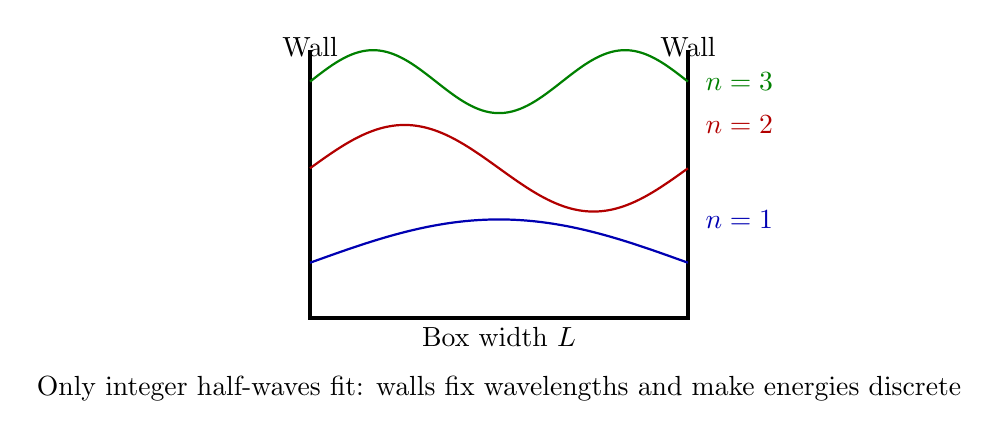
\begin{tikzpicture}[scale=1.0]
  % Infinite potential well
  \draw[very thick] (0,3.4) -- (0,0) -- (4.8,0) -- (4.8,3.4);
  \node[above] at (0,3.2) {Wall};
  \node[above] at (4.8,3.2) {Wall};
  \node[below] at (2.4,0) {Box width \(L\)};
  % n=1
  \draw[thick,blue!70!black] plot[domain=0:4.8,samples=60,smooth] (\x,{0.7+0.55*sin(180*\x/4.8)});
  \node[right,blue!70!black] at (4.9,1.25) {\(n=1\)};
  % n=2
  \draw[thick,red!70!black] plot[domain=0:4.8,samples=80,smooth] (\x,{1.9+0.55*sin(360*\x/4.8)});
  \node[right,red!70!black] at (4.9,2.45) {\(n=2\)};
  % n=3
  \draw[thick,green!50!black] plot[domain=0:4.8,samples=100,smooth] (\x,{3.0+0.4*sin(540*\x/4.8)});
  \node[right,green!50!black] at (4.9,3.0) {\(n=3\)};
  \node at (2.4,-0.9) {Only integer half-waves fit: walls fix wavelengths and make energies discrete};
\end{tikzpicture}
\end{center}

\begin{center}
\begin{tikzpicture}[scale=1.0]
  % Packet spreading
  \draw[thick,blue!70!black] plot[domain=-2.4:2.4,samples=80,smooth] (\x,{1.8*exp(-3*\x*\x)});
  \node[above,blue!70!black] at (0,1.8) {Now: narrow and tall};
  \draw[thick,red!70!black,dashed] plot[domain=-4.5:4.5,samples=100,smooth] (\x,{0.55*exp(-0.3*\x*\x)});
  \node[red!70!black] at (3.2,1.15) {\shortstack{Later: broad\\and short}};
  \draw[-{Stealth[length=2.5mm]},thick,gray] (1.5,0.9) -- (2.6,0.6);
  \draw[-{Stealth[length=2.5mm]},thick,gray] (-1.5,0.9) -- (-2.6,0.6);
  \node at (0,-0.8) {\shortstack{Free packet: wavelength-dependent phase rates\\necessarily spread the bump over time}};
\end{tikzpicture}
\end{center}

\begin{center}
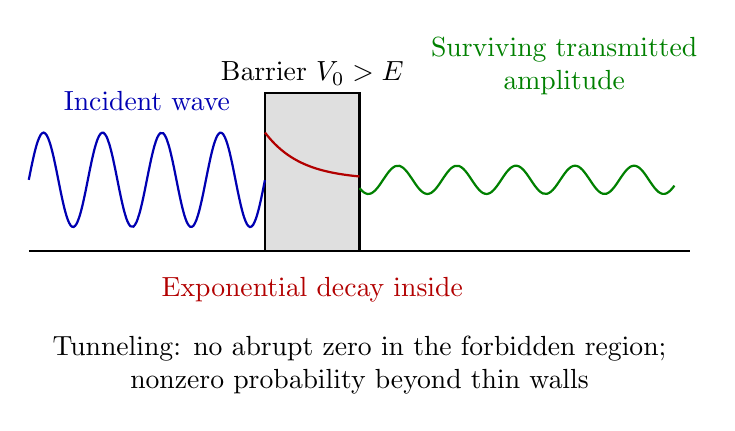
\begin{tikzpicture}[scale=1.0]
  % Barrier
  \fill[gray!25] (3,0) rectangle (4.2,2.0);
  \draw[thick] (0,0) -- (8.4,0);
  \draw[thick] (3,0) -- (3,2.0) -- (4.2,2.0) -- (4.2,0);
  \node at (3.6,2.25) {Barrier \(V_{0}>E\)};
  % Incident wave
  \draw[thick,blue!70!black] plot[domain=0:3,samples=80,smooth] (\x,{0.9+0.6*sin(480*\x)});
  \node[blue!70!black] at (1.5,1.9) {Incident wave};
  % Decay within the wall
  \draw[thick,red!70!black] plot[domain=3:4.2,samples=30,smooth] (\x,{0.9+0.6*exp(-2.2*(\x-3))});
  \node[red!70!black] at (3.6,-0.5) {Exponential decay inside};
  % Transmitted wave
  \draw[thick,green!50!black] plot[domain=4.2:8.2,samples=80,smooth] (\x,{0.9+0.18*sin(480*\x)});
  \node[green!50!black] at (6.8,2.35) {\shortstack{Surviving transmitted\\amplitude}};
  \node at (4.2,-1.45) {\shortstack{Tunneling: no abrupt zero in the forbidden region;\\nonzero probability beyond thin walls}};
\end{tikzpicture}
\end{center}

\begin{mathbridge}
The full one-dimensional Schrödinger equation is
\[
  i\hbar\,\frac{\partial\psi}{\partial t}
  =\hat{H}\psi,\qquad
  \hat{H}=-\frac{\hbar^{2}}{2m}\frac{\partial^{2}}{\partial x^{2}}+V(x).
\]
The left is state change in time. The right's second spatial derivative measures curvature: sharper means shorter wavelength and larger momentum. With \(V(x)\), it accounts fully for energy across space and shape. Insert free-particle \(V=0\) plane wave \(\psi=e^{i(kx-\omega t)}\). The left gives \(\hbar\omega\), the right \(\hbar^{2}k^{2}/(2m)\), precisely \(E=p^{2}/(2m)\). Free evolution exactly restores the classical kinetic relation, again meeting constraint three.

Separate variables to find stationary states: \(\psi(x,t)=\varphi(x)\,e^{-iEt/\hbar}\) cancels time factors, leaving the \emph{time-independent Schrödinger equation}
\[
  \hat{H}\varphi=E\varphi .
\]
Seek special shapes the Hamiltonian merely multiplies; the multiplier \(E\) is energy. Box boundaries \(\varphi(0)=\varphi(L)=0\) yield \(\varphi_{n}(x)=\sqrt{2/L}\,\sin(n\pi x/L)\) and \(E_{n}=n^{2}h^{2}/(8mL^{2})\), rigorously deriving the half-wave argument. Since \(e^{-iEt/\hbar}\) always has unit modulus, \(|\psi|^{2}\) freezes. Overall idle rotation is factorization, not metaphor. Combining the equation and its conjugate to calculate \(\partial|\psi|^{2}/\partial t\) gives a spatial flow difference: probability moves but total amount stays fixed, thanks to \(i\) on the left.
\end{mathbridge}

\begin{challenge}
Why \emph{first-order} time and \emph{complex} numbers? Conservation underlies both. A second-order wave equation needs both present wavefunction and its time derivative, enlarging the state and violating Chapter~43's wavefunction completeness. First order makes present determine future, inheriting Newtonian complete-state tradition. Complex numbers and \(i\) ensure \emph{unitary} evolution: \(\psi(t)=e^{-i\hat{H}t/\hbar}\psi(0)\), with operator \(U(t)=e^{-i\hat{H}t/\hbar}\) preserving state overlaps, hence probability. Another result: any observable commuting with the Hamiltonian, Chapter~46's language, has unchanging expectation. Energy, momentum, and angular-momentum conservation wear new clothes but none disappears. Finally a boundary: \(p^{2}/(2m)\) is low-speed kinetic energy. Near light speed, Chapter~40's true energy--momentum relation cannot fit; the equation needs a full upgrade, Chapter~49's Dirac equation.
\end{challenge}

\step{The Model's Limits}

\begin{mainline}
\textbf{Boundary one: nonrelativistic approximation.} Kinetic \(p^{2}/(2m)\) works far below light speed and fails systematically near it. High energies, heavy-atom inner electrons, and antimatter require Chapter~49's relativistic quantum theory.

\textbf{Boundary two: do not blindly equate Hamiltonian and total energy.} Precisely, the \emph{Hamiltonian} generates evolution. Only time-independent potential and an isolated system make it conserved total energy. Time-varying external fields, such as laser-driven atoms, still generate evolution through it but need not conserve system energy: atoms absorb from light. Universal identification with conserved total energy is a common conceptual misuse.

\textbf{Boundary three: no direct wavefunction measurement.} Laboratory accounts contain squared moduli, probability distributions, and phase \emph{differences}, fringe positions. Overall phase is unmeasurable. Rotating phase speaks the model's language; changing relative phases make testable facts. This matters especially for stationary states.

\textbf{Boundary four: measurement is outside this chapter.} Schrödinger describes smooth, reversible, probability-conserving evolution \emph{between} measurements. Measurement updates, collapse, use another rule examined in Chapter~45. Applying the equation to measurement itself or demanding it alone explain a unique outcome oversteps its scope.

Four further common misuses:

\begin{itemize}[leftmargin=1.8em]
  \item \emph{Stationary means motionless.} False. Probability \(|\psi|^{2}\) freezes, not motion. Box-ground energy \(E_{1}>0\) is entirely kinetic inside \(V=0\): unmoving landscape, restless undercurrents. Question three is (b).
  \item \emph{Tunneling digs a route through a wall with negative kinetic energy.} False. The route is a misleading name; negative wall-interior kinetic energy forces classical bookkeeping onto quantum mechanics. No measurement corresponds to that quantity. Measuring position inside changes the state through interaction, Chapter~45, no longer observing the original evolution.
  \item \emph{Spreading packets mean fattening particles.} False. Each detection still gives a whole electron at a point. The region where it might be found broadens, not its physique.
  \item \emph{Quantum mechanics requires discrete energy.} False. Free energies are continuous. Discreteness comes from boundaries, walls, closed orbits, periodicity. Levels belong to confinement, not quantum mechanics' default setting.
\end{itemize}
\end{mainline}

\step{Explaining the Opening Phenomenon}

\textbf{Quantum-dot televisions.} Box pricing \(E_{n}=n^{2}h^{2}/(8mL^{2})\) settles it: shrink six nanometers to three and quantized energy quadruples, pushing red toward blue-green. Material sets the intrinsic-gap base price, size the surcharge. Your screen is one stationary Schrödinger equation illuminated a hundred million times. Both opening and first guess are settled.

\textbf{Notes that never detune.} Why does hydrogen red endure ten billion years and light-years? Its electrons occupy the Coulomb potential's natural box, solved in Chapter~52. One equation and potential uniquely fix stationary levels: every hydrogen atom solves the same problem. Transitions release level differences, \(f=\Delta E/h\), creating the universe's most stable scale. Strontium clocks instrument this stability. Stationary atoms never tire from travel like springs or forks: their constancy is exact in the equation, not engineering compromise. Our most precise clocks pledge this guarantee: \emph{definite-energy components only rotate phase uniformly}.

\textbf{Three tunneling accounts.} First, USB and solid-state drives confine electrons in oxide-walled floating gates. Thick barriers exponentially suppress escape for roughly ten-year storage. Slight thinning or damage dramatically increases leakage, underpinning finite write endurance and eventual data loss. Second, scanning tunneling microscopes move fine tips close across samples. Vacuum forms a barrier; current depends exponentially on distance, changing about an order of magnitude per 0.1 nanometer. Single-atom topography becomes clear, even letters written in atoms. Third, the Sun: core proton energies of roughly a thousand electronvolts face Coulomb barriers of millions. Classically it cannot ignite; exponential tunneling gives tiny nonzero chances to meet and fuse into helium. Small probabilities sustain slow, stable burning. This 4.6-billion-year lamp has an exponentially decaying wavefunction for a wick.

\step{Thought Experiments and Challenges}

\begin{thought}[A Person in an Infinite Well]
Confine a \(70\)-kilogram person in a rigid \(1\)-meter box. From \(E_{1}=h^{2}/(8mL^{2})\),
\[
  E_{1}=\frac{(6.63\times10^{-34})^{2}}{8\times70\times1^{2}}\approx8\times10^{-70}\ \text{J},
\]
the restless speed is \(v=\sqrt{2E_{1}/m}\approx5\times10^{-36}\) meters per second. Crossing a hair's width takes about \(10^{23}\) years, a trillion universe ages. Turning a page does roughly \(10^{-2}\) joules of work, enough to reach \(n\approx10^{34}\), where relative neighboring-level spacing is only order \(10^{-33}\), effectively continuous. Quantization never disappears macroscopically; absurdly small \(h^{2}\) hides its grid beyond instruments. Classical mechanics is a distant view of densely packed \(E_{n}\), not error.
\end{thought}

\begin{thought}[Turning the Sun's Tunneling Knob]
Transmission depends exponentially on barrier width, and solar protons occupy its steep section. Imagine both directions. Increase probability a millionfold: fuel burns fiercely in antiquity, stars die before planets cool or observers evolve. Decrease it a millionfold: protons never cross, the Sun never lights, and Earth freezes. We sit beside a star already shining 4.6 billion years with another five billion ahead partly because this exponential slope permits slow stability. The same mechanism works beside your bones: smoke-detector americium-241 releases \(\alpha\) particles by nuclear tunneling at a constant rate. Radioactive half-life is constant escape probability per unit time integrated into exponential decay. From wager to retirement, tunneling quietly manages the world's timetable.
\end{thought}

\begin{puzzles}
\item A box electron jumps from \(n=2\) to \(n=1\), emitting light. Double box width with everything else fixed: how many times the original wavelength results? \emph{Hint}: write \(\Delta E=E_{2}-E_{1}=3h^{2}/(8mL^{2})\), inspect the power of \(L\), then convert energy to wavelength, not frequency.
\item Equal portions of box ground \(E_{1}\) and first excited \(E_{2}\) states make left- and right-half probabilities oscillate. What determines frequency? Does doubling \(E_{2}-E_{1}\) speed or slow it? \emph{Hint}: each phase rotates at \(\omega=E/\hbar\); cross terms sense only their \emph{difference}, like tuning-fork beats.
\item Thicker flash insulation preserves data longer, but writing and erasing through tunneling need higher voltage, slower operation, and potentially greater damage. Why does slight thickening have large effects at both ends? \emph{Hint}: exponentials. Ten-percent thickness change may shift probability by orders of magnitude; this world has no gentle adjustments.
\item A reader says unchanging box-ground probability means zero kinetic energy, contradicting \(E_{1}=h^{2}/(8mL^{2})\). What is confused? \emph{Hint}: with zero potential, what energy is \(E_{1}\)? Does stationarity freeze \(|\psi|^{2}\) or the wavefunction? Has an unchanged-modulus rotating complex number not moved?
\end{puzzles}

Quantum mechanics' main machine is assembled: Chapter~43 supplied states and Born readings; this chapter supplied the between-measurement Schrödinger engine. Two rooms remain unexplored: Chapter~45 reconciles continuous evolution with one measurement outcome and examines updates; Chapter~46 abstracts wavefunctions into vectors and Hamiltonians into operators, revealing \(\hat{H}\varphi=E\varphi\) as an eigenvalue/eigenvector problem and linear algebra as the native language. Quantum dots, atomic clocks, flash memory, and the Sun are one machine idling or working in different settings.
